\documentclass{beamer}

\usepackage{beamerthemesplit}
\usepackage{graphicx,url}
\usepackage[brazil]{babel}
\usepackage[utf8]{inputenc}

\mode<presentation>
{
  \usetheme{Marburg}
  \setbeamercovered{transparent}
}

\newcommand{\eng}[1]{\textit{#1}}
\newcommand{\goiaba}{\textit{Goiaba}}
\newcommand{\code}[1]{\texttt{#1}}

\title{Goiaba---um software para processar contornos}
\author{Marcos Sampaio}
\date{14 de novembro de 2008}

\logo{\includegraphics[scale=.15]{logo-genos}}

\begin{document}

\frame{\titlepage}

\section{Introdução}

\subsection{Definições}

\frame{
  \frametitle{Contornos em Música}
  \begin{figure}
    \centering
    \includegraphics[scale=.9]{5a-sinfonia}
  \end{figure}

  \begin{figure}
    \centering
    \includegraphics[scale=1.4]{c-3120}
  \end{figure}
}

\frame{
  \frametitle{Semelhança e coerência}
  \begin{figure}
    \centering
    \includegraphics{ly-2031}
    \hspace{1em}
    \includegraphics[scale=1.4]{c-2031}
  \end{figure}
}

\subsection{O que e por que?}

\frame{
  \frametitle{Objetivo e justificativas}
  \begin{itemize}
  \item Justificativa
    \begin{itemize}
    \item Coerência
    \item Manipulação por operações
    \item Estudos escassos
    \end{itemize}
  \item Objetivo
    \begin{itemize}
    \item Software para processar contornos
    \end{itemize}
  \end{itemize}
}

\subsection{Representações}

\frame{
  \frametitle{Representações de contornos}
  \begin{itemize}
  \item Representação simbólica
    \begin{itemize}
    \item Contorno: Z(2 0 3 1)
    \item Elementos: Z$_0=2$, Z$_1=0$, Z$_2=3$ e Z$_3=1$
    \end{itemize}
  \item Representação gráfica
    \begin{figure}
      \centering
      \includegraphics[scale=1.5]{c-2031}
    \end{figure}
  \end{itemize}
}

\frame{
  \frametitle{Representação de operações}
  \begin{itemize}
  \item Retrógrado de X(1 2 3): $retr(X(1\;2\;3))=Y(3\;2\;1)$
  \item Transposição de X(1 2 3) com fator 2: $transp(X(1\;2\;3)\;2)=W(3\;4\;5)$
  \item Concatenação de operações: $transp(retr(inv(rot(X(1\;2\;3))\;2))\;3)$
  \end{itemize}
}

\subsection{Operações}

\frame {
  \frametitle{Operações implementadas}
  \begin{enumerate}
  \item Retrogradação
  \item Inversão
  \item Transposição
  \item Rotação
  \item Expansão de intervalos
  \item Classe de contornos
  \item Série de contornos adjacentes
  \item Vetor de séries de contornos
  \item Vetores I e II de classes de contorno
  \item Matriz de comparação
  \end{enumerate}
  (ver no Goiaba)
}

 \frame {
  \frametitle{Retrógrado e inversão}
  \begin{table}
    \centering
    \begin{tabular}{r|lll}
      Contorno & Retrógrado & Inversão & Retrógrado da inversão \\
      \hline
      (5 9 6 8) & (8 6 9 5) & (5 1 4 2) & (2 4 1 5) \\
      (5 7 6 8) & (8 6 7 5) & (5 3 4 2) & (2 4 3 5) \\
      (3 1 5 0) & (0 5 1 3) & (3 5 1 6) & (6 1 5 3)
    \end{tabular}

  \begin{columns}[t]
    \column{3cm}
    \begin{figure}
      \centering
      \includegraphics[scale=.7]{c-5968}
      \caption{Original}
    \end{figure}

    \column{3cm}
    \begin{figure}
      \centering
      \includegraphics[scale=.7]{c-8695}
      \caption{Retrógrado}
    \end{figure}

    \column{3cm}
    \begin{figure}
      \centering
      \includegraphics[scale=.7]{c-5142}
      \caption{Inversão}
    \end{figure}
  \end{columns}
  \end{table}
}

\frame {
  \frametitle{Transposição e rotação}
  \begin{tabular}{r|lll}
    Contorno & Rotação 1 & Rotação 2 & Rotação 3 \\
    \hline
    (5 9 6 8) & (9 6 8 5) & (6 8 5 9) & (8 5 9 6)
  \end{tabular}
}

\frame {
  \frametitle{Expansão de intervalos}
\;\;$expan(P(5\;9\;6\;8)\;2)=Q(5\;13\;7\;11)$
\begin{figure}
  \centering
  \includegraphics[scale=.5]{expansao}
\end{figure}
}
\section{O Goiaba}

\frame{
  \frametitle{Desenvolvimento}
  \begin{itemize}
  \item Common Lisp \cite{graham94:lisp} e SBCL
  \item Metodologia bottom-up
  \item Orientação a objetos
  \end{itemize}
}

\frame{
  \frametitle{Representações}
  \begin{itemize}
  \item Contornos simples: \code{(5 9 6)}
  \item Contornos com duração: \code{((0 5)(1 9)(2 6))}
  \end{itemize}
  (ver no Goiaba)
}

\frame{
  \frametitle{Classes e macros}
  \begin{itemize}
  \item \texttt{ponto}: \code{(x y)}\\
    \code{\#p(x y)}
  \item \texttt{contorno-simples}: \code{(y w)}\\
    \code{\#s(y w)}
  \item \texttt{contorno-duracao}: \code{((x y) (z
      w))}\\
    \code{\#d(\#p(x y) \#p(x y))}
  \end{itemize}
}

\begin{frame}[fragile]
  \frametitle{Funções}
  \footnotesize
\begin{verbatim}
(defmethod transpor ((objeto contorno-duracao) fator)
  (map-contorno-duracao #L(transpor !1 fator) (pontos objeto)))

(defmethod transpor ((objeto contorno-simples) fator)
  (map-contorno-simples #L(+ !1 fator) (pontos objeto)))
\end{verbatim}
  \normalsize
\end{frame}

\begin{frame}[fragile]
  \frametitle{Plotagem}
  \begin{itemize}
  \item Biblioteca cl-pdf
  \end{itemize}  

\begin{verbatim}
(let ((contorno #s(0 5 3 4 1 3)))
  (simple-plot
   contorno "original" :blue
   (transpor contorno 2) "transposição" :green
   (retrogradar contorno) "retrógrado" :red
   (inverter contorno) "inversão" :orange
   (rotacionar contorno 1) "rotação" :darkcyan
   ))
\end{verbatim}
\end{frame}

\frame{
  \frametitle{Resultado da plotagem}

  \begin{figure}
    \centering
    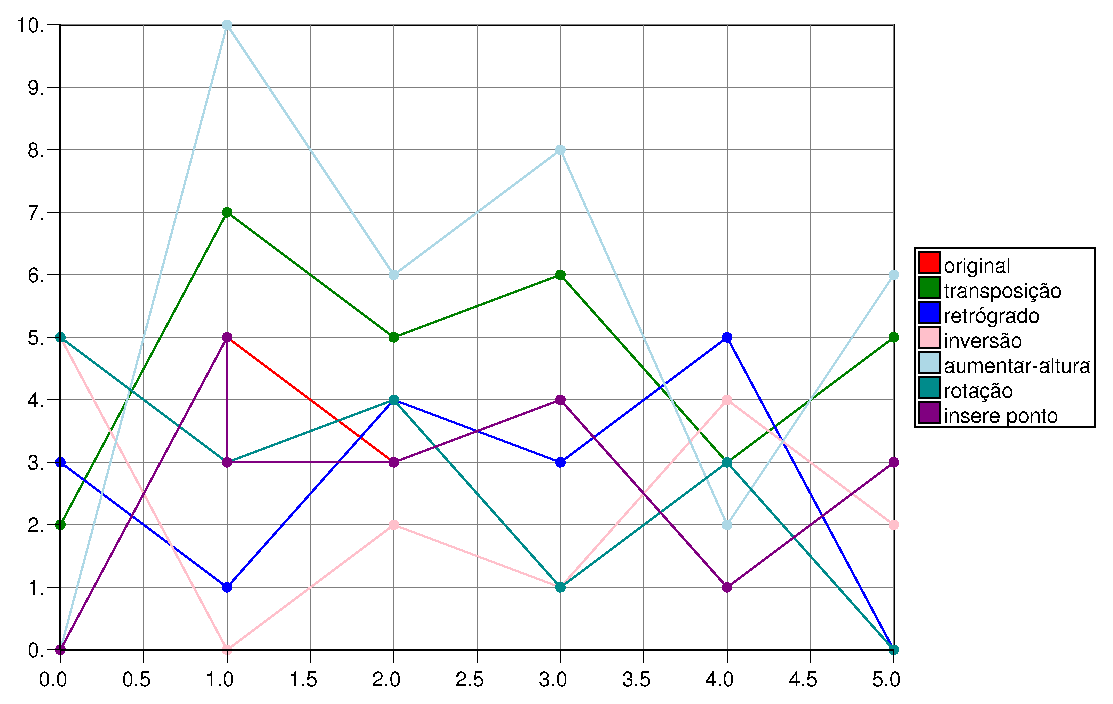
\includegraphics[scale=.5]{contornos}
    \caption{Saída do Goiaba}
  \end{figure}
}

\section{Conclusões}

\frame{
  \frametitle{Discussão}
  \begin{itemize}
  \item Programação como metodologia de estudo
  \end{itemize}
}

\frame{
  \frametitle{Trabalhos futuros}
  \begin{itemize}
  \item Implementar conversão em/de partituras musicais
  \item Implementar interface gráfica
  \item Lançar versão estável
  \end{itemize}
}

\frame{
  \frametitle[allowframebreaks]{Referências}
  \bibliographystyle{alpha}
  \bibliography{melodic-contour,music-perception,composition,music-harmony-and-theory,programs,music-analysis,audio,genos,computer-science}
}

\end{document}
